\documentclass[sigplan,11pt,nonacm]{acmart}
\settopmatter{printfolios}

\usepackage{booktabs} % For formal tables
\usepackage{subcaption}
\usepackage{tikz}
\usepackage{pgfplots}
\usepackage{pgfplotstable}
\usepackage{hyphenat}
\usepackage{todonotes}
\usepackage[babel]{csquotes}


\begin{document}
\title{Utilizing Parallel Workers: \\LLVM's Vectorization Plan}
\author{Jonas Fritsch}
\affiliation{%
  \institution{Technical University of Munich}
}
\email{jonas.fritsch@tum.de}

\begin{abstract}
Lorem ipsum
\end{abstract}

\maketitle

%%%%%%%%%%%%%%%%%%%%%%%%%%%%%%%%%%%%%%%%%%%%%%%%%%%%%%%%%%%%%%%%%%%%%%%%%%%%%%%%%%%%%%%%%%%%%%%%%%%%%%


\section{Introduction}
\label{sec:introduction}
Modern CPUs are often equipped with multiple different vector registers. These registers are nowadays 
as wide as 512 bits, allowing for the processing of multiple data streams at once (SIMD). By 
batching multiple values together in one register, different ISAs like Intel AVX or ARM SVE allow 
the execution of the same instruction for all values in a vector register simultaneously. 
Utilizing this leads to significant performance improvements over the scalar equivalent most of 
the time.

However, as manual code vectorization can quickly become very time-consuming, especially when
supporting different CPU architectures, modern compilers aim to automatically transform scalar code
to use vectorization when applicable.

As one of the most widely used compilation frameworks, LLVM~\cite{10.5555/977395.977673} has 
implemented and refined its auto-vectorization over many years. It provides two different 
Vectorizers, one for innermost loops (LoopVectorize) and one for super-word parallelism 
(SLPVectorize)~\cite{llvmvec}.

This system, however, had quite a few limitations, as the loop vectorizer could only handle
innermost loops and neither outer loops, complex control flow, nor non-inlined functions. 
Additionally, while multiple different vectorizations for the same scalar code 
would be possible, the current vectorizers working directly on the LLVM IR could not model
and compare the costs of such different vectorization approaches.

With these limitations in mind, Intel started an ongoing refactorization effort to migrate LLVM's
auto-vectorization pipeline to utilize a more abstract Vectorization Plan 
(VPlan)~\cite{llvmextloopvec,llvmvplan}. The final goal would be to unite LLVM's auto-vectorization
in a single flexible system capable of optimizing SLPs, inner, and nested loops with complex 
control flows. The auto-vectorization pass would create, compare, and transform multiple different 
VPlans, each modeling a different vectorization approach, and finally materialize the best one into
the LLVM IR.

LLVM's VPlan is currently being integrated into the existing Loop Vectorizer and is
already modeling most inner loop vectorizations and transformations. Vectorization for outer 
loops is also in development and can be enabled by setting the \texttt{-enable-vplan-native-path} 
flag~\cite{llvmouterloop}. In the future, the plan will be to merge both of these loop vectorization
paths into one.


%%%%%%%%%%%%%%%%%%%%%%%%%%%%%%%%%%%%%%%%%%%%%%%%%%%%%%%%%%%%%%%%%%%%%%%%%%%%%%%%%%%%%%%%%%%%%%%%%%%%%%


\section{Background}
\label{sec:background}
Modern SIMD ISAs like Intel AVX, ARM NEON or even vector-length agnostic ISAs like ARM SVE provide
a variety of different instructions to allow vectorization of even complex control flows. To lower
the complexity for implementing auto-vectorization, the general optimizations are often divided
into different categories:

\subsection{Inner Loop Vectorization}
Innermost loops are loops whose body's control flow does not contain any loops, bound or unbound.
Vectorizing such loops is generall eas

\begin{figure}
  \centering
  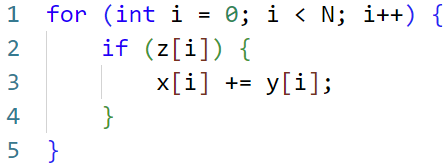
\includegraphics[width=0.35\textwidth]{images/inner-loop-vec.png}
  \caption{asdf}
  \label{fig:inner-loop-vec}
\end{figure}

\subsection{Super-Word Parallelism (SLP) Vectorization}
asdf

\subsection{Outer Loop Vectorizaton}
asdf

\subsection{Function Vectorization}
asdf

\subsection{Vectorization Constraints}
asdf


%%%%%%%%%%%%%%%%%%%%%%%%%%%%%%%%%%%%%%%%%%%%%%%%%%%%%%%%%%%%%%%%%%%%%%%%%%%%%%%%%%%%%%%%%%%%%%%%%%%%%%


\section{LLVM's Vectorization Plan}
\label{sec:vplan}
Lorem ipsum


%%%%%%%%%%%%%%%%%%%%%%%%%%%%%%%%%%%%%%%%%%%%%%%%%%%%%%%%%%%%%%%%%%%%%%%%%%%%%%%%%%%%%%%%%%%%%%%%%%%%%%


\section{Related Work}
\label{sec:relatedwork}
Lorem ipsum


%%%%%%%%%%%%%%%%%%%%%%%%%%%%%%%%%%%%%%%%%%%%%%%%%%%%%%%%%%%%%%%%%%%%%%%%%%%%%%%%%%%%%%%%%%%%%%%%%%%%%%


\section{Summary and Future Work}
\label{sec:summary}
Lorem ipsum


%%%%%%%%%%%%%%%%%%%%%%%%%%%%%%%%%%%%%%%%%%%%%%%%%%%%%%%%%%%%%%%%%%%%%%%%%%%%%%%%%%%%%%%%%%%%%%%%%%%%%%

\bibliographystyle{ACM-Reference-Format}
\bibliography{paper} % read paper.bib file

\end{document}
